\documentclass{article}

\usepackage[english]{babel}
\usepackage[style=abnt,backend=biber,citecounter=true,backrefstyle=three]{biblatex}
\addbibresource{sample.bib}
\usepackage[letterpaper,top=2cm,bottom=2cm,left=3cm,right=3cm,marginparwidth=1.75cm]{geometry}
\usepackage{float}

\usepackage{amsmath}
\usepackage{graphicx}
\usepackage[colorlinks=true, allcolors=blue]{hyperref}

\title{Trabalho OpenMP: Algoritmo Bitonic Sort}
\author{Henrique Utzig e Pedro Afonso Klein}

\begin{document}
\maketitle

\section{Introdução}

O presente documento é o relatório do primeiro trabalho da disciplina INF01008 - Programação Paralela e Distribuída no semestre 2025/1. Nesse trabalho, os integrantes do grupo deveriam escolher um algoritmo que já foi questão da Maratona de Programação Paralela \cite{MPP}, avalia-lo e paraleliza-lo (se possível). Além disso, o grupo executou uma série de testes com ambas implementações, sequencial e paralela, e a análise e comparação destes testes será apresentada em seguida.

O algoritmo escolhido pelo grupo foi Bitonic Sort da décima Maratona de Programação Paralela (2015) \cite{BitonicSort}.

\section{O Algoritmo Bitonic Sort}

O Bitonic Sort é um algoritmo de ordenação baseado em comparações, originalmente desenvolvido para arquiteturas de rede de interconexão paralela. Ele é especialmente eficiente quando o número de elementos a serem ordenados é uma potência de dois. O algoritmo organiza os dados em sequências bitônicas — sequências que primeiramente crescem e depois decrescem, ou vice-versa — e então aplica uma operação de \textit{merge} específica para produzir a ordenação final.

\subsection{Funcionamento}

O algoritmo começa dividindo recursivamente a sequência em duas metades: a primeira é ordenada em ordem crescente e a segunda em ordem decrescente. Em seguida, aplica-se o processo de \textit{bitonic merge} para transformar essa sequência bitônica em uma sequência totalmente ordenada.

A função \texttt{recBitonicSort} realiza a construção das subsequências bitônicas. Esta função chama a \texttt{bitonicMerge} para fazer a fusão entre as subsequências. As comparações e trocas entre pares de elementos são feitas pela função \texttt{compare}, que realiza a troca condicionalmente à direção (ascendente ou descendente).

\subsection{Características Paralelizáveis}

O Bitonic Sort possui um alto grau de paralelismo devido à sua estrutura regular e previsível. Em cada etapa de comparação e troca, pares independentes de elementos podem ser processados simultaneamente. As chamadas recursivas, tanto na fase de construção quanto na fase de mesclagem, são ideais para paralelização.

\section{Implementação Paralela}

A implementação paralela do Bitonic Sort foi realizada utilizando a biblioteca OpenMP, que permite a criação de regiões paralelas com facilidade através de diretivas como \texttt{\#pragma omp parallel} e \texttt{\#pragma omp task}.

\subsection{Modificações no Código}

Duas funções principais foram paralelizadas:

\begin{itemize}
  \item \texttt{recBitonicSortParallel}: versão paralela da função de construção das subsequências bitônicas. As chamadas recursivas são envolvidas por diretivas \texttt{\#pragma omp task} com a diretiva condicional \texttt{if (cnt > task\_threshold)}, permitindo o controle do overhead da criação de tarefas.
  \item \texttt{bitonicMergeParallel}: versão paralela da função de mesclagem. As chamadas recursivas também foram paralelizadas com \texttt{\#pragma omp task}. Foi testado o uso de paralelismo no \textit{loop} de comparações com \texttt{\#pragma omp parallel for}, porém observou-se degradação de desempenho, motivo pelo qual essa diretiva foi comentada.
\end{itemize}

A função \texttt{bitonicSortParallel} inicia a execução paralela encapsulando a chamada à função recursiva dentro de uma região \texttt{single} para garantir que a construção das tarefas seja feita por apenas uma \texttt{thread} mestre.

% Adicionar os trechos no relatório talvez seja uma boa, mas acho que esse aqui não agrega muito
% \subsection{Trecho de Código Relevante}

% \begin{verbatim}
% #pragma omp parallel
% {
%     #pragma omp single
%     {
%         recBitonicSortParallel(0, N, ASCENDING);
%     }
% }
% \end{verbatim}

% Essa estrutura garante que todas as tarefas geradas nas chamadas recursivas possam ser executadas de forma concorrente pelas demais \texttt{threads} disponíveis.

\subsection{Parâmetro de Controle de Paralelismo}

Para evitar a criação excessiva de tarefas com granularidade muito pequena (o que poderia causar overhead e perda de desempenho), foi utilizado o parâmetro \texttt{task\_threshold}. Somente quando o número de elementos a ser ordenado for maior do que esse valor, novas tarefas são criadas.


\section{Metodologia de Testes}

Para avaliar o comportamento dos algoritmos, foram executados testes sistemáticos nas versões sequencial e paralela do Bitonic Sort, bem como nas versões sequencial e paralela do Merge Sort. A inclusão do Merge Sort serve como referência, pois sua estrutura difere do Bitonic Sort apenas na rotina de fusão (\emph{merge}), que também foi paralelizada no Bitonic Sort. Dessa forma, é possível comparar diretamente o impacto da paralelização em dois algoritmos de ordenação com complexidade e padrões de acesso de memória semelhantes.```


\subsection{Testes Iniciais}

Foram conduzidos testes preliminares para avaliar incrementalmente a eficácia das diretivas do OpenMP aplicadas ao problema do \textit{bitonic sort}. Esses testes iniciais foram executados de maneira exploratória, comparando manualmente o tempo de execução ao introduzir diferentes diretivas e ajustes de paralelização. A partir dessas primeiras avaliações, foi obtida uma versão inicial considerada estável o suficiente para ser submetida a testes mais rigorosos e sistemáticos.

\subsection{Testes em Lote Automatizados}

Após validar a eficácia inicial das diretivas de paralelização, foi desenvolvido um script em Python para automatizar e sistematizar a execução dos testes em lote. Esse script executa o programa compilado diversas vezes, variando os seguintes parâmetros:

\begin{itemize}
\item \textbf{Tamanho do Input (N)}: foram utilizados arquivos de entrada contendo de $2^0$ (1 elemento) até $2^{24}$ (16.777.216 elementos). Esses inputs são strings aleatórias de 7 caracteres geradas por um script auxiliar.
\item \textbf{Número de Threads}: determinado automaticamente pelo script, iniciando no número máximo disponível na máquina (40 threads na hype) e reduzindo pela metade sucessivamente até alcançar a execução sequencial com uma única thread.
\item \textbf{Threshold de paralelização (task threshold)}: testado especificamente nas versões paralelas, com valores pré-definidos de 1024, 2048 e 4096 para analisar o impacto do overhead de criação de tarefas. A escolha destes valores foi feita durante os testes manuais, mas foi realizado também um teste especifico para threshold, confirmando as escolhas.
\end{itemize}

Cada configuração foi executada cinco vezes para permitir o cálculo da média e do desvio padrão dos tempos de execução, garantindo maior confiabilidade estatística dos resultados obtidos.

Todos os testes foram realizados em um nodo da máquina \textit{hype PCAD}. A configuração específica de execução incluiu ainda a variável de ambiente \texttt{OMP\_PROC\_BIND=TRUE}, garantindo a fixação das threads aos núcleos físicos para evitar interferências causadas por trocas de contextos de threads durante a execução.

Ao final de cada execução, outro script auxiliar validava automaticamente a correção dos resultados, verificando se as strings estavam corretamente ordenadas, assegurando assim a validade funcional do algoritmo além de seu desempenho temporal.

Os resultados de todos esses testes foram coletados em arquivos CSV para posterior análise gráfica e estatística detalhada, permitindo comparações diretas entre diferentes métodos de ordenação (sequencial e paralelo, bitonic e mergesort) sob diferentes cargas e configurações.

\section{Resultados e Analise}

Nesta seção apresentamos a análise dos resultados obtidos por meio da ferramenta Intel VTune Profiler e dos testes automatizados em lote, avaliando o desempenho das versões sequenciais e paralelas dos algoritmos Bitonic Sort e Merge Sort.

\subsection{Análises do VTune}

Idealmente, gostaríamos de examinar os hotspots e a distribuição de threads por meio das análises \emph{hotspots} e \emph{threading} do Intel VTune Profiler, mas não foi possível coletar essas métricas. Em vez disso, realizamos dois perfis utilizando o tipo de análise \emph{hpc‐performance}: um para a versão sequencial e outro para a versão paralela executada com 40 threads na máquina \textit{hype}. Esses testes forneceram uma visão comparativa do comportamento de baixo nível (CPI, utilização de núcleos, pressões de memória e cache) em ambos os cenários.```

\subsubsection{Análise da Versão Sequencial}

\begin{figure}[H]
    \centering
    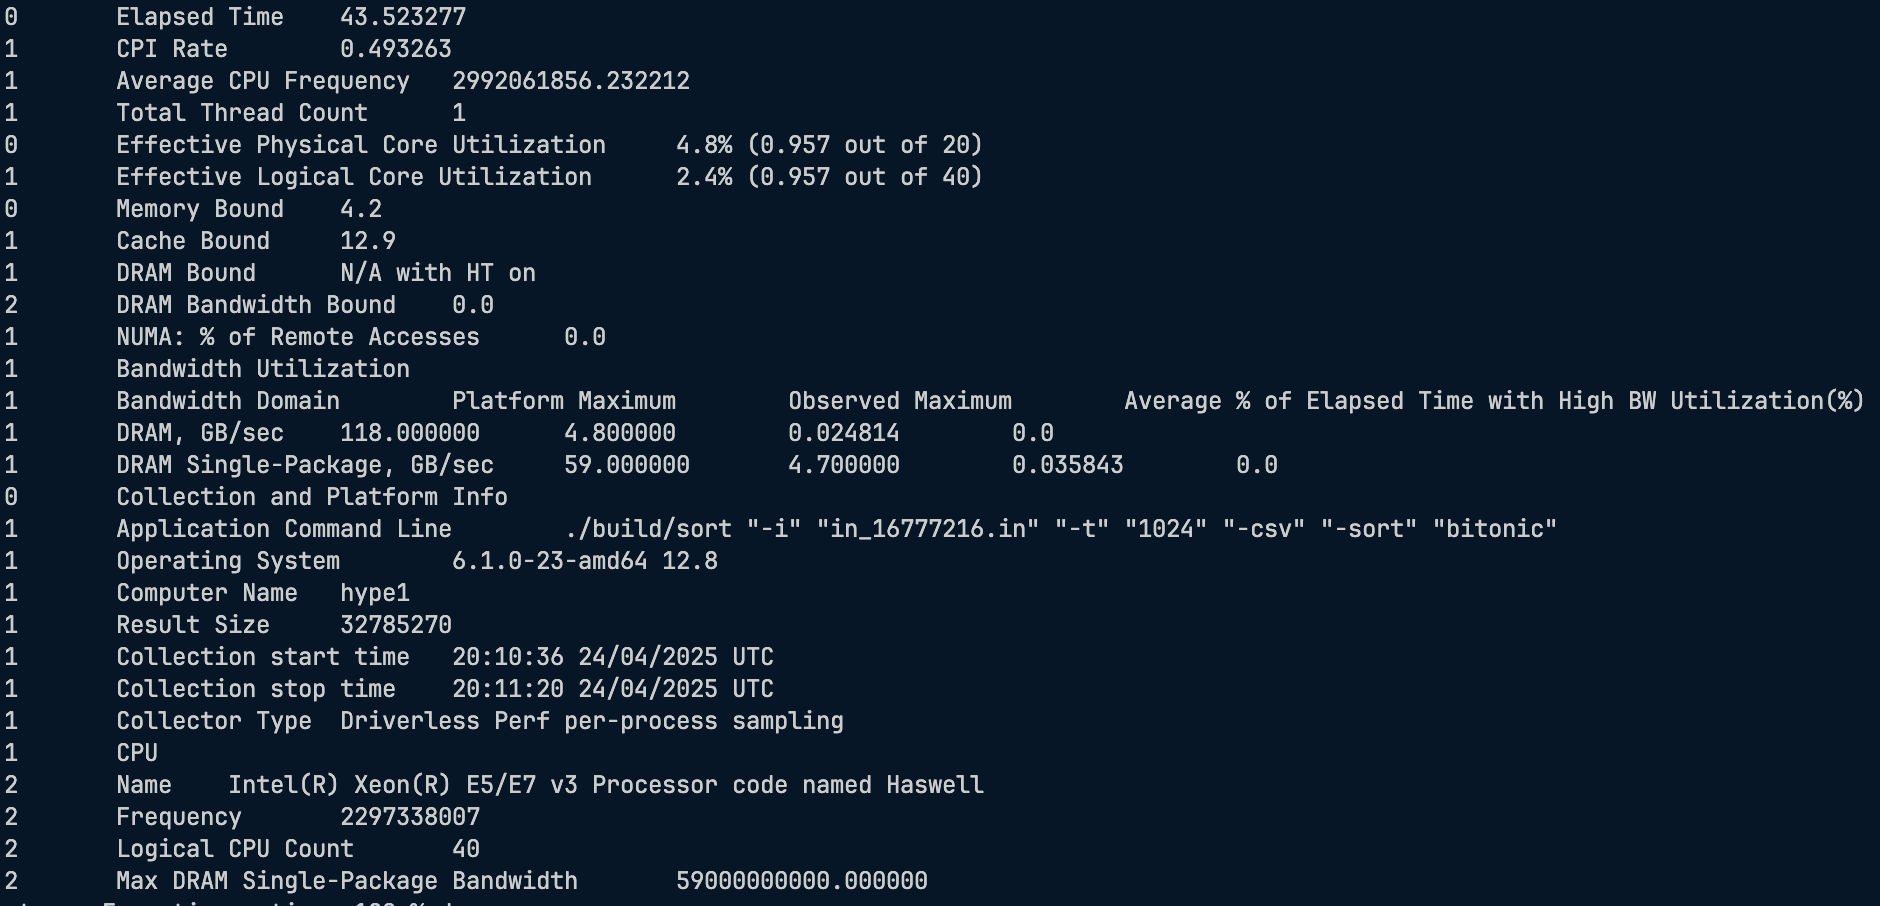
\includegraphics[width=0.8\linewidth]{images/vtune_sequential.png}
    \caption{Resultados da analise hpc-performance do vtune com programa sequencial e 16777216 entradas}
    \label{fig:vtune_sequential}
\end{figure}

A versão sequencial apresentou tempo de execução de aproximadamente 43,52 s para $N = 16\,777\,216$ elementos, com CPI médio de 0,49, indicando boa eficiência em nível de instrução. Porém, a utilização efetiva dos núcleos físicos ficou em apenas 4,8 \%, refletindo o caráter estritamente sequencial do algoritmo. O indicador \emph{Memory Bound} atingiu 4,2 \%, e o \emph{Cache Bound} 12,9 \%, mostrando certa dependência da hierarquia de memória, enquanto a banda DRAM chegou a apenas 4,8 GB/s, fração mínima da capacidade disponível.

\subsubsection{Análise da Versão Paralela}

\begin{figure}[H]
    \centering
    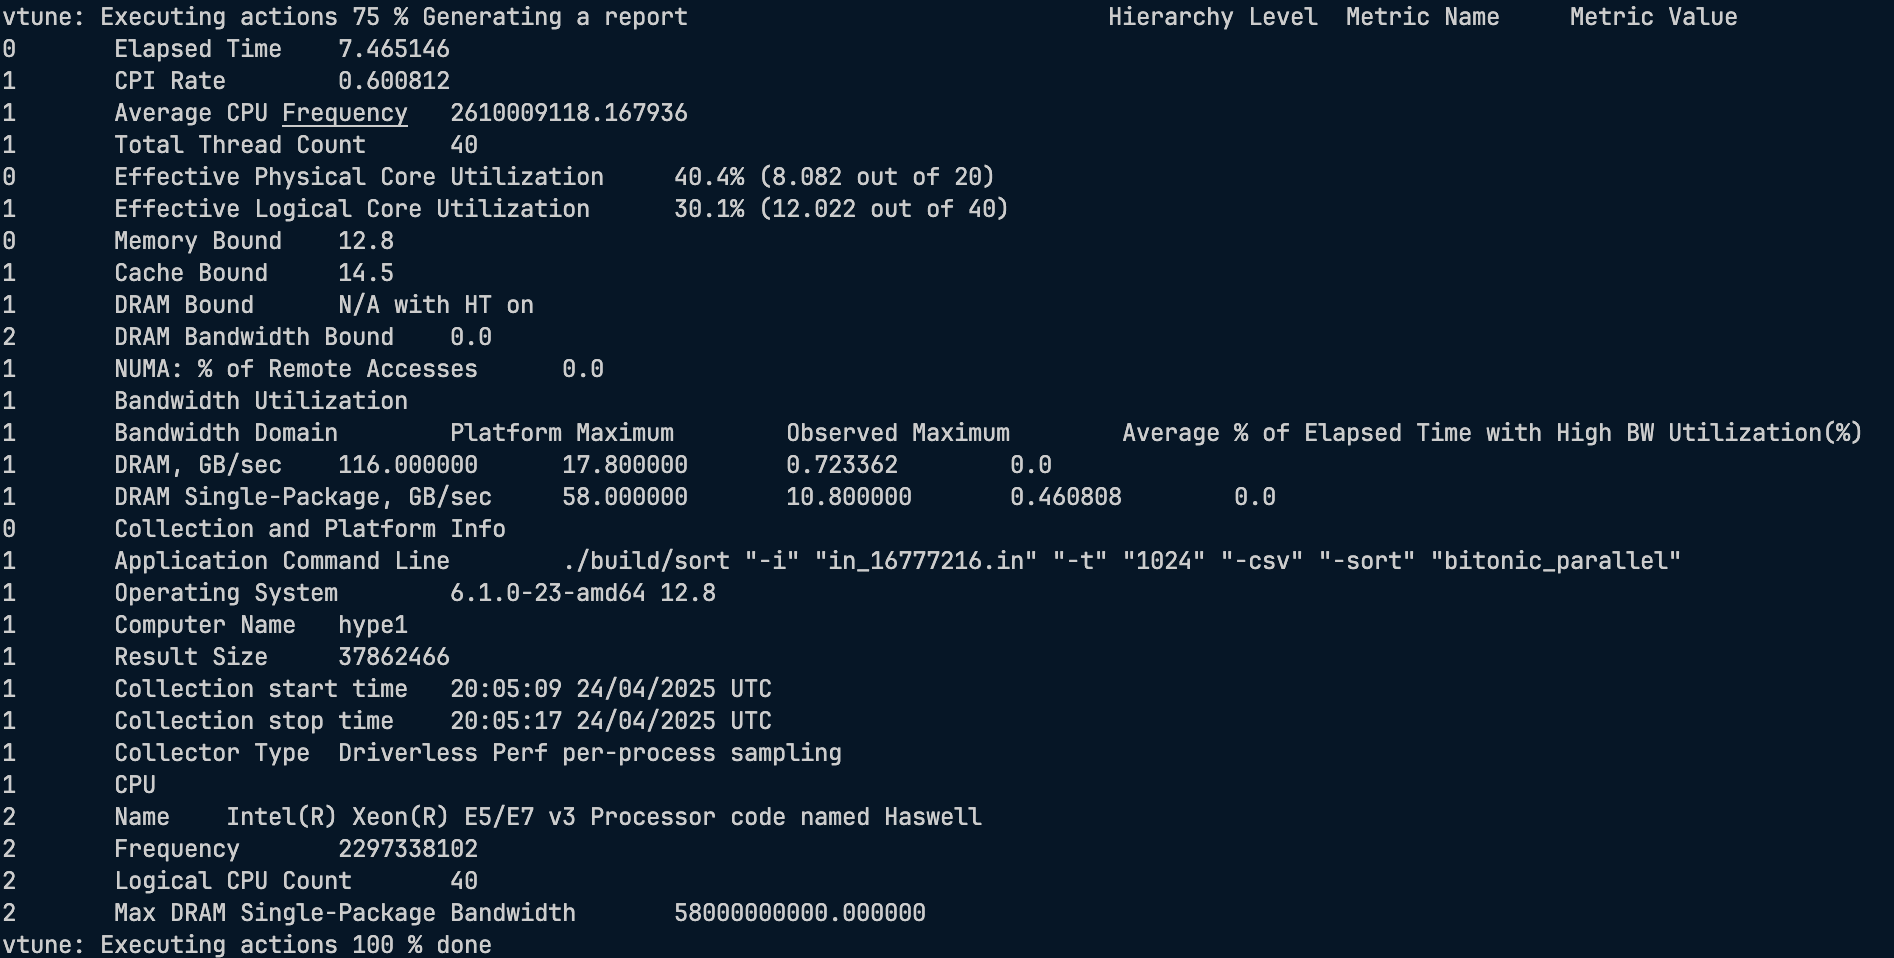
\includegraphics[width=0.8\linewidth]{images/vtune_parallel.png}
    \caption{Resultados da analise hpc-performance do vtune com 40 threads e 16777216 entradas}
    \label{fig:vtune_parallel}
\end{figure}

Com paralelismo em 40 threads, o tempo total caiu para cerca de 7,47 s — um speedup de 5,8× em relação à versão sequencial. Observou‐se aumento do CPI para 0,60, sugerindo overhead de paralelização, e a utilização física dos núcleos atingiu 40,4 \% (aprox. 8 núcleos ativos), evidenciando sincronizações e gerenciamento de tarefas. O \emph{Memory Bound} subiu para 12,8 \% e o \emph{Cache Bound} para 14,5 \%, indicando maior pressão sobre cache, enquanto a banda DRAM alcançou 17,8 GB/s, ainda distante do teto de 116 GB/s.

\subsubsection{Comparação}

Embora o paralelismo proporcione ganhos expressivos de desempenho, existe sobrecarga significativa no gerenciamento de tarefas que limita a eficiência de uso dos recursos e aumenta a pressão sobre a memória cache. Fica claro que a paralelização só se justifica plenamente em cargas de trabalho grandes, onde o overhead é amortizado.

\subsection{Resultados dos testes automatizados}

\begin{figure}[H]
    \centering
    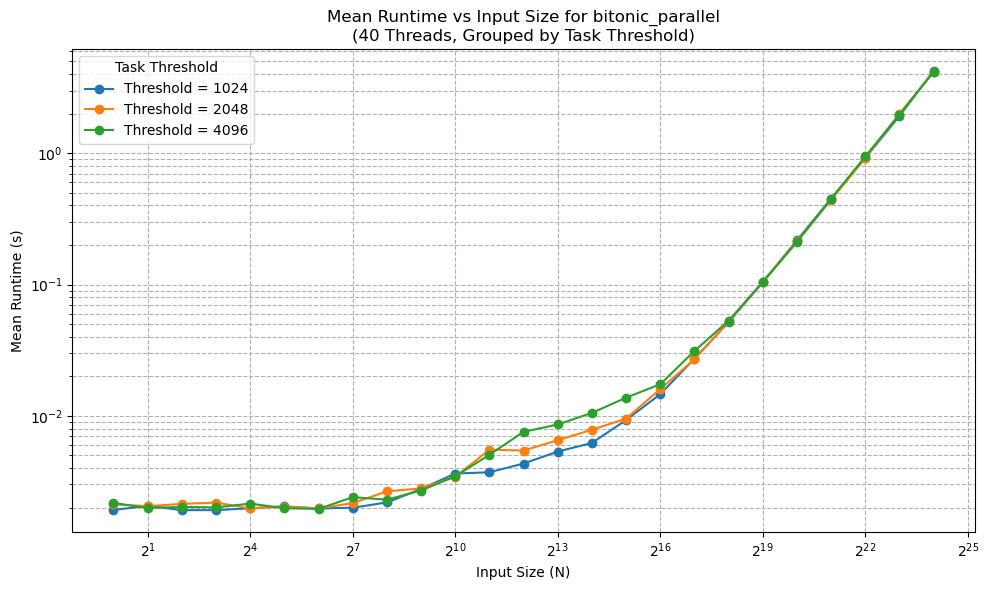
\includegraphics[width=0.8\linewidth]{images/threshold_comp1.png}
    \caption{Tempo de execução vs entrada com diferentes thresholds para bitonic sort paralelo}
    \label{fig:thresholdByInput}
\end{figure}

A Figura~\ref{fig:thresholdByInput} mostra o tempo médio de execução do Bitonic Sort paralelo em função do tamanho do input para diferentes thresholds (1024, 2048 e 4096), usando 40 threads. O threshold de 1024 apresentou ligeira vantagem em entradas maiores, mas o ganho se estabiliza conforme $N$ cresce, sugerindo a necessidade de ajustes de granularidade de acordo com a entrada.

\begin{figure}[H]
    \centering
    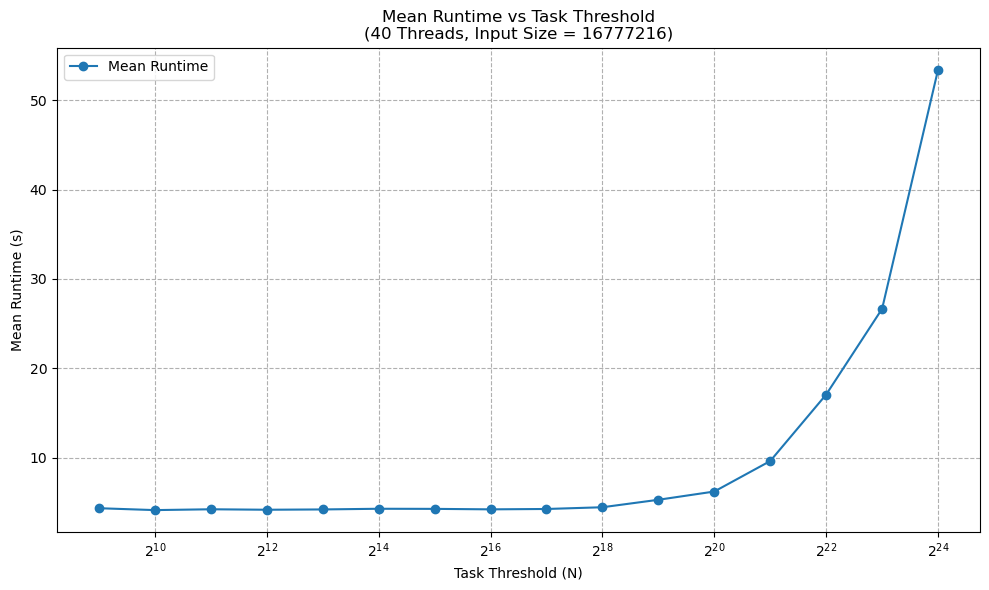
\includegraphics[width=0.8\linewidth]{images/threshold.png}
    \caption{Tempo de execução vs diferentes thresholds para bitonic sort}
    \label{fig:enter-label}
\end{figure}

A Figura~\ref{fig:enter-label} ilustra o efeito do threshold variando de 512 até 16 777 216 para um input fixo. Observa-se que, além de um valor mínimo, o desempenho se torna pouco sensível a thresholds menores, indicando que o ponto ótimo depende do tamanho do input.

\begin{figure}[H]
    \centering
    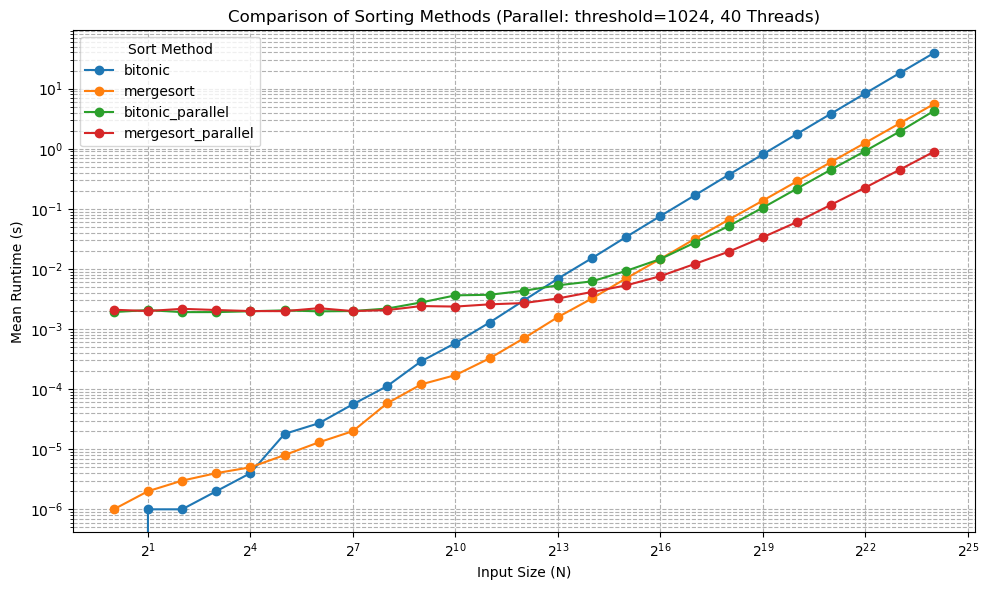
\includegraphics[width=0.8\linewidth]{images/byInput.png}
    \caption{Tempo de execução vs entrada para diferentes tipos de sort}
    \label{fig:sortsByInput}
\end{figure}

Na Figura~\ref{fig:sortsByInput} comparamos os quatro métodos (bitonic e merge, seqüencial e paralelo) em diferentes tamanhos de entrada, com threshold de 1024 e 40 threads. Os algoritmos sequenciais levam vantagem para entradas pequenas devido ao overhead de paralelização, enquanto as versões paralelas só ultrapassam as sequenciais após o threshold. O Merge Sort paralelo mostrou-se  mais rápido que o Bitonic Sort paralelo no intervalo testado.

\begin{figure}[H]
    \centering
    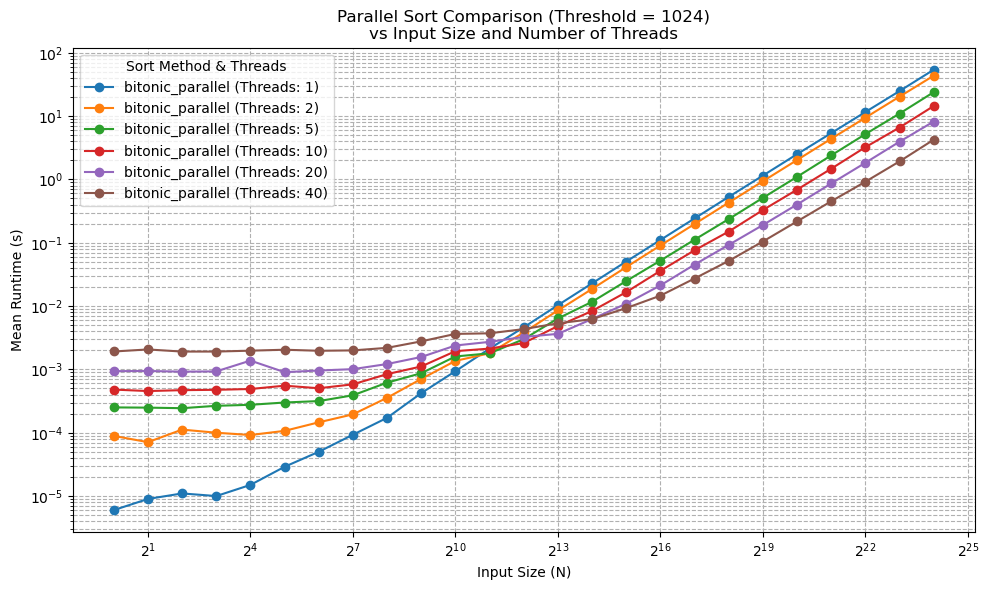
\includegraphics[width=0.8\linewidth]{images/byInputAndThreads.png}
    \caption{Tempo de execução vs entrada para diferente números de threads para bitonic sort paralelo}
    \label{fig:threadsByInput}
\end{figure}

A Figura~\ref{fig:threadsByInput} evidencia a escalabilidade do Bitonic Sort paralelo para diferentes números de threads (1, 2, 5, 10, 20 e 40), com threshold de 1024. O speedup cresce com o número de threads, mas somente para entradas maiores que o threshold — tarefas muito finas geram overhead e penalizam o desempenho.

\begin{figure}[H]
    \centering
    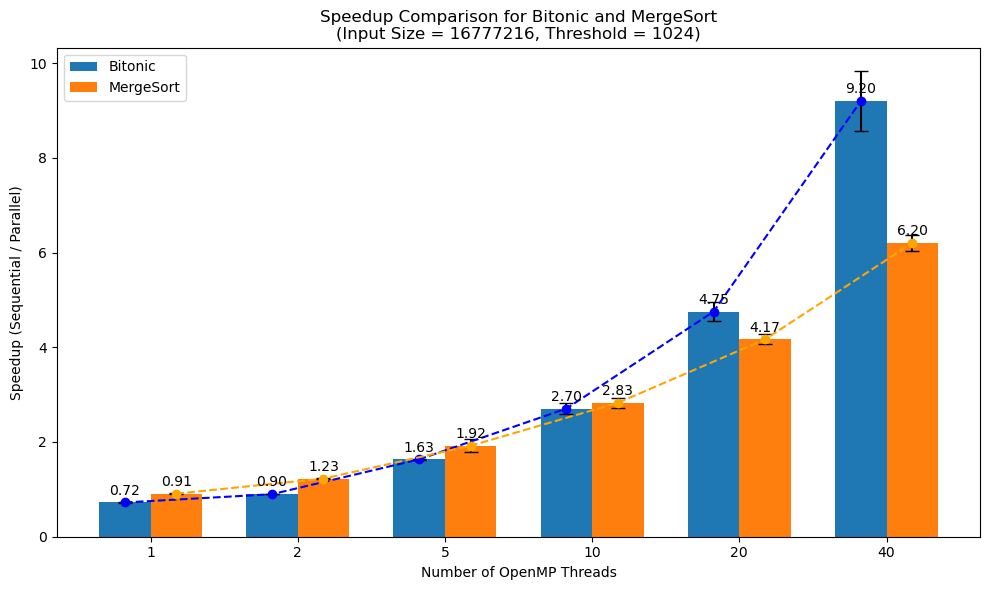
\includegraphics[width=0.8\linewidth]{images/speedup.png}
    \caption{Speedup de acordo com numero de threads entre merge a bitonic sort}
    \label{fig:speedup}
\end{figure}

Por fim, a Figura~\ref{fig:speedup} compara o speedup entre Merge Sort paralelo e Bitonic Sort paralelo, incluindo barras de desvio-padrão. Apesar do Merge Sort apresentar menor variabilidade e leve vantagem em speedup moderado, o Bitonic Sort tende a escalar melhor para níveis elevados de paralelismo, sinalizando maior potencial em arquiteturas com mais núcleos ou unidades de execução especializadas, como GPUs ou até mesmo hardware especifico.

\section{Conclusao}

Este trabalho demonstrou que a paralelização do Bitonic Sort com OpenMP proporciona ganhos de desempenho expressivos (até 9,2×), mas sofre overhead considerável na criação e sincronização de tarefas. O parâmetro \texttt{task\_threshold} mostrou-se crítico: 1024 foi um valor eficiente para as configurações testadas, embora o ponto ótimo varie conforme o tamanho da entrada. Em comparação, o Merge Sort paralelo superou o Bitonic Sort em cenários de paralelismo moderado, mas o Bitonic Sort apresenta maior potencial de escalabilidade quando há mais threads disponíveis.

Para trabalhos futuros podemos melhorar os seguintes fatores:
\begin{itemize}
  \item Implementar threshold adaptativo baseado no tamanho de cada subproblema;
  \item Explorar estratégias de afinidade de threads e \emph{NUMA} para reduzir overhead de sincronização;
  \item Otimizar a localidade de dados, minimizando miss de cache e pressões de memória;
  \item Avaliar modelos híbridos de paralelismo (por exemplo, combinar \texttt{task} com \texttt{parallel for}) e extensões para aceleração em GPUs ou hardware especializado.
\end{itemize}

Em síntese, a estrutura regular do Bitonic Sort o torna interessante para sistemas com alto grau de paralelismo, mas seu desempenho depende de ajustes finos de granularidade e gestão de memória compartilhada.

\printbibliography

\end{document}
